\chapter{Studi Literatur}


\section{Pasar Saham Indonesia}
Gagasan mengenai pasar saham dapat ditelusuri berabad-abad yang lalu, bermula dari bentuk-bentuk awal perdagangan komoditas dan obligasi pemerintah, hingga menjadi platform canggih yang saat ini memfasilitasi pertukaran ekuitas perusahaan. Salah satu contoh awal dari sistem pasar yang relatif terorganisasi muncul pada abad ke-17 di Amsterdam dengan Perusahaan Hindia Timur Belanda (VOC), yang dianggap sebagai perusahaan publik pertama di dunia \parencite{Petram2014,Neal1990}. Di sini, para investor dapat membeli dan menjual saham pada satu lokasi terpusat. Ini menjadi cikal bakal bursa saham modern  \parencite{Neal2005,Goetzmann2016}. Seiring waktu, gagasan ini menyebar ke seluruh Eropa, dengan munculnya pasar di London dan Paris. Pada akhir abad ke-18 dan awal abad ke-19, Bursa Efek New York (NYSE) muncul di Amerika Serikat dan menjadi fondasi bagi jaringan global pasar keuangan yang saling terhubung \parencite{Markham2002,Goetzmann2016}.

Ketika industrialisasi dan globalisasi meningkat pada abad ke-20, pasar saham tumbuh semakin cepat dan komopleks. Peralihan dari platform bursa yang fisik menjadi berbasis elektronik yang dapat beroperasi lintas zona waktu dan lintas negara memungkinkan partisipasi oleh yang lebih luas, baik oleh investor institusional maupun ritel, serta meningkatkan likuiditas dan efisiensi pasar. Liberalisasi aliran modal pada paruh kedua abad tersebut, ditambah dengan kemajuan teknologi, memungkinkan negara-negara berkembang membangun pasar sahamnya sendiri. Hal ini menciptakan lanskap keuangan global yang lebih beragam dan saling terkait \parencite{OECD2018}.

Di Asia Tenggara, pasar saham memegang peran penting dalam menyalurkan modal domestik dan asing ke sektor-sektor kunci untuk mendorong pertumbuhan dan pembangunan ekonomi. Pada awalnya, pasar saham Indonesia beroperasi secara sederhana dengan jumlah perusahaan terbatas dan partisipasi investor yang minim \parencite{OJK2007}. Selama beberapa dekade, pasar ini mengalami transformasi signifikan. Pembentukan Bursa Efek Jakarta (BEJ) dan Bursa Efek Surabaya (BES) menyediakan gelangang perdagangan saham yang terpisah, meskipun keduanya sempat menghadapi tantangan dalam mencapai kedalaman (\textit{depth}) dan keluasan (\textit{breadth}) dalam menjual emiten yang tercatat. Namun, reformasi regulasi, peningkatan tata kelola perusahaan, serta penguatan kerangka hukum membantu meningkatkan kepercayaan investor dan mendekatkan pasar modal Indonesia dengan standar global \parencite{OECD2018}.

Tahun 2007 menandai titik balik penting bagi pasar modal Indonesia, ketika Bursa Efek Jakarta dan Bursa Efek Surabaya bergabung membentuk Bursa Efek Indonesia (BEI). Konsolidasi ini bertujuan merampingkan operasional, mengurangi fragmentasi, dan memperkuat daya saing di tengah arus globalisasi \parencite{OJK2007}. Bersamaan dengan reorganisasi institusional, regulator keuangan seperti Otoritas Jasa Keuangan  (OJK) menerapkan langkah-langkah untuk meningkatkan integritas pasar, transparansi, dan perlindungan investor. Upaya ini sejalan dengan praktik terbaik internasional guna mencerminkan kesadaran bahwa pasar saham yang berfungsi dengan baik sangat penting untuk menarik investasi jangka panjang, mendukung pembiayaan perusahaan, dan pada akhirnya berkontribusi pada stabilitas serta pertumbuhan ekonomi.

Bukti empiris menunjukkan bahwa peran pasar saham Indonesia terus berkembang, sejalan dengan peningkatan jumlah perusahaan yang tercatat dan diversifikasi sektor usaha—dari pertanian, barang konsumsi, keuangan, infrastruktur, hingga perusahaan berbasis teknologi. Diversifikasi ini meningkatkan ketahanan pasar, mengurangi \textit{concentration risk}, dan mendorong investor untuk melihat lanskap korporasi Indonesia secara lebih cermat. Masuknya investor asing, yang didukung oleh lingkungan regulasi yang lebih kondusif, turut menambah likuiditas. Investor lokal juga diuntungkan oleh inisiatif peningkatan literasi keuangan serta platform perdagangan yang lebih mudah digunakan \parencite{OECD2018}.

Perkembangan lain yang signifikan adalah berubahnya profil investor di Indonesia. Jika pada masa lalu pasar didominasi oleh institusi besar dan individu borjuis, kini partisipasi investor ritel semakin meningkat. Kampanye pemerintah, program edukasi, serta layanan pialang daring telah membuka akses perdagangan saham untuk segmen yang sebelumnya tidak dapat dijangkau dalam masyarakat. Demokratisasi akses ini membentuk budaya investasi yang lebih inklusif dan dapat menstabilkan pasar dengan memperluas basis atau fondasi dari modal-modal jangka panjang. Dengan demikian, pasar saham Indonesia kini tidak lagi menjadi domain eksklusif kelompok tertentu, melainkan menjadi platform tempat masyarakat umum dapat turut andil dalam perjalanan ekonomi nasional.

Meski begitu, pasar saham Indonesia tetap rentan terhadap guncangan eksternal dan volatilitas regional, yang merupakan tantangan yang biasa dihadapi oleh banyak pasar negara berkembang \parencite{torre2007emerging}. Faktor seperti fluktuasi harga komoditas global, ketegangan geopolitik, serta perubahan kebijakan moneter internasional semuanya dapat memengaruhi sentimen investor dan aliran modal \parencite{BloomEtAl2019}. Faktor domestik—termasuk perubahan kebijakan pemerintah, indikator makroekonomi, dan standar tata kelola perusahaan—juga berinteraksi membentuk dinamika pasar. Walaupun pasar saham Indonesia telah matang dan terintegrasi dengan keuangan global, ia tetap beroperasi dalam ekosistem kompleks yang memerlukan pengelolaan risiko yang berkelanjutan (IMF, 2022).

Upaya untuk meningkatkan infrastruktur pasar, menerapkan kerangka regulasi yang kokoh, serta mengadopsi inovasi teknologi yang lebih canggih akan semakin memperkuat posisi Indonesia sebagai tujuan investasi utama di Asia Tenggara. Kemungkinan pengenalan instrumen keuangan yang lebih beragam, integrasi yang lebih dalam dengan pasar modal internasional, serta penerapan teknologi digital mutakhir seperti perdagangan algoritmik dapat membawa era baru efisiensi dan transparansi. Di saat yang sama, faktor Lingkungan, Sosial, dan Tata Kelola (ESG) kian menonjol, sejalan dengan tren investasi berkelanjutan di tingkat global. Hal ini yang mendorong perusahaan-perusahaan untuk memenuhi standar-standar yang lebih tinggi serta tanggung jawab korporasi, yang berpotensi menarik kelompok investor yang lebih sadar dan bertanggung jawab akan ESG.


\section{Kecerdasan Buatan}
Kecerdasan Buatan (\textit{Artificial Intelligence} atau AI) adalah cabang ilmu komputer yang bertujuan menciptakan mesin serta sistem yang mampu menjalankan tugas-tugas yang biasanya memerlukan kecerdasan manusia \parencite{RussellNorvig2020}. Bidang ini berupaya membuat komputer dapat memahami, belajar dari lingkungan, dan berinteraksi dengan cara yang menyerupai atau bahkan melampaui kemampuan kognitif manusia dalam mengenali pola, mengambil keputusan, dan memecahkan masalah tanpa kita sebagai manusia perlu memberitahu mesin secara eksak apa yang perlu mereka lakukan.

Sejak kemunculannya sebagai disiplin akademik pada pertengahan abad ke-20, AI telah dipengaruhi oleh berbagai bidang ilmu, seperti matematika, psikologi, linguistik, biologi, filsafat, serta rekayasa komputer. Pendekatan awal riset AI banyak berfondasi pada \textit{symbollic logic} dan aturan-aturan eksplisit yang meniru proses berpikir manusia \parencite{RussellNorvig2020}. Namun, seiring waktu, AI berkembang dengan memasukkan metode statistik dan pendekatan berbasis data, termasuk pembelajaran mesin (\textit{machine learning}). Pembelajaran mesin memungkinkan sistem meningkatkan kinerjanya melalui pengalaman secara iteratif \parencite{Goodfellow-et-al-2016}. Salah satu cabang pembelajaran mesin yang menonjol adalah pembelajaran mendalam (\textit{deep learning}), yang memanfaatkan jaringan saraf buatan yang terinspirasi oleh struktur dan fungsi otak manusia, untuk mengenali pola dalam data yang kompleks.

Saat ini, AI telah diterapkan pada berbagai aspek kehidupan sehari-hari, mulai dari asisten virtual berbasis suara, kendaraan otonom, sistem rekomendasi, hingga analisis data tingkat lanjut pada bidang-bidang sains lainnya. Dalam sektor-sektor seperti kesehatan, keuangan, manufaktur, dan pendidikan, AI dapat meningkatkan efisiensi, produktivitas, serta kualitas pengambilan keputusan. Meskipun perkembangan AI melaju pesat, isu tentang etika, transparansi, dan akuntabilitas tetap harus diproritaskan untuk menjadi perhatian penting untuk mendorong adanya diskusi mengenai pengembangan dan penerapan AI secara bertanggung jawab agar tidak merugikan umat manusia \parencite{JobinEtAl2019}.

\section{Pembelajaran Mesin}
Pembelajaran mesin (\textit{machine learning}) adalah salah satu cabang dari kecerdasan buatan yang berfokus pada pengembangan algoritma dan model yang dapat belajar dari data tanpa secara eksplisit diprogram ulang untuk setiap tugas \parencite{Mitchell1997}. Dalam pembelajaran mesin, komputer “belajar” dengan menganalisis data dengan jumlah yang besar untuk menemukan pola atau hubungan yang kemudian dapat digunakan untuk membuat prediksi atau mengambil keputusan di masa mendatang. Pendekatan ini berbeda dari pemrograman tradisional, di mana kita menuliskan aturan secara eksplisit di dalam kode, sedangkan pada pembelajaran mesin, sistem secara otomatis menyimpulkan aturan ataupun cara untuk melakukan sebuah \textit{task} tersebut dari data.

Secara umum, pembelajaran mesin dapat dibagi menjadi tiga kategori utama: \textit{supervised learning}, \textit{unsupervised learning}, dan \textit{reinforcement learning} \parencite{Goodfellow-et-al-2016}. \textit{Supervised learning} membangun model menggunakan data yang telah dilabeli untuk “melatih” model agar dapat memprediksi label pada data baru yang belum pernah dilihat oleh model tersebut. \textit{Unsupervised learning } tidak memerlukan label karena berfokus pada eksplorasi struktur atau pola tersembunyi di dalam data tersebut. Sementara itu, \textit{reinforcement learning} menggunakan interaksi sistem dengan \textit{environment}, di mana model secara iteratif memperbarui strateginya dalam memenuhi atau melaksanakan \textit{task} berdasarkan umpan balik yang dapat berupa “reward” atau “punishment”.

Perkembangan pembelajaran mesin sangat pesat berkat ketersediaan data yang semakin melimpah dan peningkatan daya komputasi yang besar. Metode ini telah dimanfaatkan dalam berbagai bidang, seperti pengenalan suara dan wajah, klasifikasi dokumen, \textit{fraud detection}, analisis pasar saham, serta diagnosis medis berbasis citra \parencite{MohriRostamizadehTalwalkar2018}. Seiring dengan kemajuan pembelajaran mesin, tantangan dalam pembelajaran mesin juga muncul. Salah satu contohnya adalah dalam hal interpretabilitas model, privasi data, dan bias algoritma. Oleh karena itu, penelitian dan inovasi dalam pembelajaran mesin terus dilakukan untuk memastikan agar teknologi ini tetap dapat digunakan, aman, serta bermanfaat secara luas bagi masyarakat.

\section{Time Series data}
Data deret waktu (\textit{time series data}) adalah jenis data yang direkam, dikumpulkan, atau diamati secara berurutan berdasarkan dimensi waktu \parencite{Chatfield2003}. Karakteristik utama dari data deret waktu adalah adanya ketergantungan atau keterkaitan antara nilai pada suatu point waktu dengan nilai-nilai pada point-point sebelumnya. Ketergantungan ini membuat pendekatan analisis data deret waktu berbeda dengan analisis data yang tidak mengkonsiderasi urutan data.

Terdapat banyak jenis data yang disimpan dalam tipe \textit{time series}. Beberapa dari contohnya adalah harga saham harian dari sebuah perusahaan, jumlah penumpang kereta setiap bulan, tingkat inflasi tahunan, atau konsumsi energi listrik per jam. Pola yang muncul dalam data deret waktu seringkali mencerminkan proses atau fenomena mendasar yang terjadi secara dinamis, misalnya tren meningkat dan menurun ataupun pola \textit{seasonality}. Memahami dan mengetahui eksistensi dari pola-pola ini dapat membantu dalam membuat keputusan, perencanaan strategis, serta prediksi masa depan yang lebih tepat\parencite{HyndmanAthanasopoulos2018}.

Dalam analisis data deret waktu, berbagai metode statistik dan algoritma pembelajaran mesin dapat digunakan. Metode tradisional seperti \textit{Autoregressive Integrated Moving Average} (ARIMA) atau model \textit{Vector Autoregression} (VAR) telah lama diaplikasikan untuk memodelkan dan memprediksi data deret waktu, namun seiring meningkatnya kompleksitas data serta kebutuhan akan model yang lebih fleksibel, pendekatan modern seperti model jaringan saraf dan arsitektur Transformer mulai banyak diterapkan \parencite{Goodfellow-et-al-2016}. Perkembangan ini terjadi karena model-model lama seperti ARIMA maupun VAR kurang mampu mempertimbangkan efek nilai masa lalu yang sangat jauh terhadap nilai masa kini, terutama dalam interval waktu yang panjang, sehingga diperlukan model yang dapat mempelajari pola non-linear dan hubungan dependensi jangka panjang.

 
\section{Neural Network}

Dikembangkannya \textit{neural network} sebagai salah satu solusi untuk membuat \textit{artificial intelligence} terinspirasi dari munculnya ide bahwa kecerdasan manusia  serta struktur otak manusia tidak memiliki karakteristik yang sama seperti komputer (need citation). Otak manusia tidak bekerja secara \textit{rigid} seperti komputer. Otak manusia dapat bekerja secara adaptif apabila terdapat informasi baru yang datang. Hal ini disebabkan oleh sifat \textit{neuroplasticity} dari otak ( need citation).


    \begin{figure}[H]
        \centering
        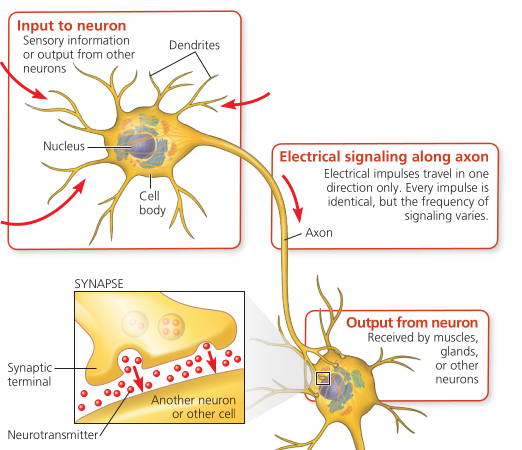
\includegraphics[width=0.5\textwidth]{resources/chapter-2-biological-neuron.png}
        \caption{  \textit{Biological neuron}\parencite{orr2021biology}}  
        \label{fig:biological-neuron}   
    \end{figure}
 
Pada gambar \ref{fig:biological-neuron}, informasi didapatkan melalui \textit{dendrites}. Setelah itu, informasi akan diolah oleh \textit{nucleus} lalu akan diteruskan oleh \textit{axon}. \textit{Axon} akan menentukan seberapa besar signal yang sudah diolah oleh \textit{nucleus} akan diteruskan ke neuron - neuron lainnya.

Konsep neuron tersebut dicoba dititru oleh ilmuwan - ilmuwan ilmu komputer. Kecerdasan buatan dapat dimodelkan sebagai sebuah grap dengan \textit{artificial neural network} yang terdiri dari \textit{input nodes}, \textit{computing nodes}, dan \textit{output nodes}. Fungsi dari \textit{input nodes} adalah hanya sebagai \textit{node} yang akan melakukan propagasi informasi dari \textit{node} itu sendiri menuju ke \textit{computing nodes}. Pada \textit{computing node}, akan terjadi komputasi. Setelah itu, informasi akan dipropagasikan lagi sampai menuju \textit{output nodes}. Ketiga tipe \textit{node} tersebut direpresentasikan di gambar \ref{fig:graph-neural-network} dimana \textit{input nodes} terdapat pada \textit{input layer}, \textit{computing nodes} terdapat pada \textit{hidden layer}, dan \textit{output nodes} terdapat pada \textit{output layer}. 

    \begin{figure}[H]
         \centering
        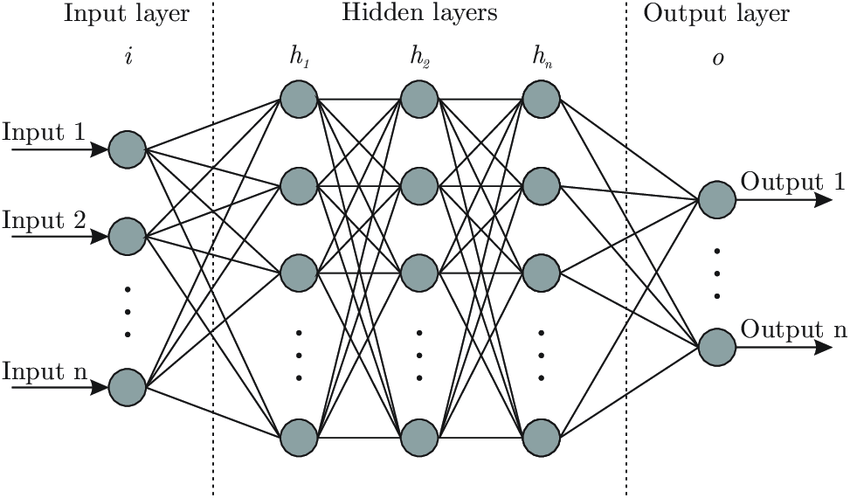
\includegraphics[width=0.8\textwidth]{resources/chapter-2-neural-network-graph.png}
        \caption{Graf \textit{Neural Network}.\parencite{towardsdatascienceNeuralnetworks}}  
        \label{fig:graph-neural-network}
    \end{figure}

Fungsi dari \textit{input nodes} dan \textit{output nodes} sudah \textit{self-explanatory} dimana kedua jenis \textit{node} tersebut hanya untuk sebagai pempropagasi informasi dan penyimpan hasil kalkulasi \textit{computing node}. \textit{Computing node} atau yang sering juga disebut dengan \textit{perceptron} memiliki struktur yang berbeda. Pada gambar \ref{fig:perceptron-neural-network}, \textit{computing node} berindeks $K$ dapat direpresentasikan sebagai sebuah neuron yang menerima $M$ buah \textit{input} dari dendritnya. Pertama-tama, akan datang $M$ buah sinyal melalui dendrit dari neuron tersebut. Setiap dendrit pada \textit{computing node} memiliki \textit{weight} yang merupakan rasio dari seberapa besar informasi dari dendrit tersebut berkontribusi kepada neuron tersebut yang dapat disimbolkan sebagai $W_{k,i}$. Perlu juga ditambahkan sebuah variabel \textit{bias} yang agnostik terhadap hasil perhitungan pada \textit{layer sebelumnya}. Variabel ini dapat kita simbolkan sebagai sinyal yang datang dari dendrit dengan indeks ke 0 dengan \textit{weight} 1. Semua sinyal tersebut akan dimasukkan ke dalam \textit{summing function} pada \ref{eq:summing-function}. 

    \begin{figure}[H]
         \centering
        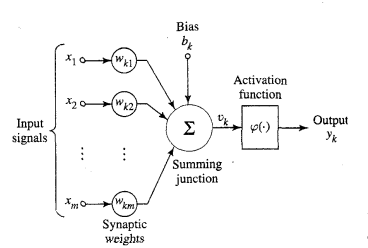
\includegraphics[width=0.8\textwidth]{resources/chapter-2-nonlinear-neuron.png}
        \caption{Perceptron buatan \parencite{haykin1998neural}}  
        \label{fig:perceptron-neural-network}
    \end{figure}

\begin{equationfloat}
\begin{equation}
\vec{v_k} = \sum_{i=0}^M w_i x_i  
\end{equation}
\caption{\textit{Summing Function}}
\label{eq:summing-function}
\end{equationfloat}


Nilai yang telah didapatkan dari \textit{summing function} akan lanjut diproses oleh \textit{activation function}. \textit{Activation function} disimbolkan sebagai \( \left| \phi(\cdot) \right| \)  pada gambar \ref{fig:perceptron-neural-network}. \textit{Activation function} akan menerima input lalu akan mengubahnya menjadi nilai pada \textit{range} \( [0,N] \). \textit{Activation function} diperlukan guna untuk mengatasi ketidaklinearitasan data seperti pada gambar \ref{fig:non-linear-data}. Apabila hasil \textit{summing function} tidak diproses lebih lanjut menggunakan \textit{activation function}, maka semua hasil komputasi hanyalah sebuah proses \textit{matrix multiplication} yang tidak dapat mengatasi ketidaklinearitasan data.Salah satu \textit{activation function} yang paling banyak digunakan adalah  ReLU (\textit{Rectified Linear Unit}) \textit{function} yang ada pada persamaan \ref{eq:ReLU}. ReLU banyak digunakan sebagai \textit{activation function} dikarenakan ReLU tidak akan mengalami \textit{vanishing gradient} ketika model melakukan \textit{backward pass} dalam \textit{training weights} dari dendrit setiap neuron.



\begin{equationfloat}
\begin{equation}
\text{ReLU}(x) =
\begin{cases} 
x, & \text{if } x > 0 \\
0, & \text{if } x \leq 
\end{cases}
\end{equation}
\caption{\textit{Rectified Linear Unit Function}}
\label{eq:ReLU}
\end{equationfloat}

    \begin{figure}[H]
         \centering
        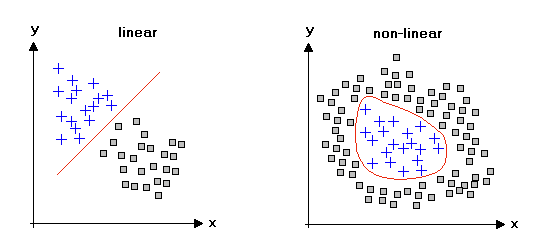
\includegraphics[width=0.8\textwidth]{resources/chapter-2-non-linearity-data.png}
        \caption{Data non-linear \parencite{nonlineargraph}}  
        \label{fig:non-linear-data}
    \end{figure}

Untuk setiap iterasi \textit{pass neural network}, akan dikalkulasikan sebuah nilai menggunakan \textit{loss function}. Semakin tinggi nilai dari \textit{loss function}, maka semakin buruk model tersebut bekerja. Terdapat banyak sekali tipe dari \textit{loss function}. Salah satunya adalah \textit{Mean Squared Error} seperti pada persamaan \ref{eq:MSE}. \textit{Loss Function} akan mengambil nilai pada \textit{layer} terakhir atau \textit{output layer} lalu melakukan komparasi untuk mencari tahu seberapa jauh model \textit{drifted} dari prediksinya.  

\begin{equationfloat}
\begin{equation}
\text{MSE} = \frac{1}{n} \sum_{i=1}^{n} (y_i - \hat{y}_i)^2
\end{equation}
\caption{\textit{Mean Squared Error}}
\label{eq:MSE}
\end{equationfloat}

Secara umum, satu iterasi dalam \textit{training neural network} terdiri atas 2 tahap yaitu \textit{forward pass} dan \textit{backward pass}. \textit{Forward pass} akan melakuka propagasi informasi dari \textit{input layer} menuju ke \textit{output layer} dimana akan terjadi komputasi pada setiap neuron yang dilewati. Setelah itu, akan dilakukan komputasi performa model menggunakan \textit{loss function}. \textit{Loss function} ini nantinya akan digunakan pada saat \textit{backward pass} dimana \textit{weight} dari setiap dendrit di neuron akan dikalkulasi ulang respektif terhadap nilai dari \textit{loss function}. \textit{Training} dari model \textit{neural network} terjadi pada saat \textit{backward pass} ini. 

\subsection{Recurrent Neural Network}
RNN merupakan jenis \textit{neural network} yang dirancang untuk memproses data sekuensial dengan mempertahankan informasi dari waktu sebelumnya. \textit{Vanilla neural network} tidak peduli dengan urutan sekuens data sehingga semua data itu dikonsiderasi sebagai sama.

\subsubsection{Vanilla RNN}
textbf{Recurrent Neural Network (RNN)} secara umum adalah jenis \textit{neural network} yang dirancang untuk memproses data secara sekuensial. Pada RNN, informasi tidak hanya mengalir dari lapisan \textit{input} ke lapisan \textit{output}, tetapi juga “diputar kembali” (\textit{recurred}) ke dalam \textit{hidden state} yang memungkinkan jaringan menyimpan konteks dari waktu ke waktu. Arsitektur RNN dapat dilihat pada gambar \ref{fig:RNN-architecture}

    \begin{figure}[H]
        \centering
        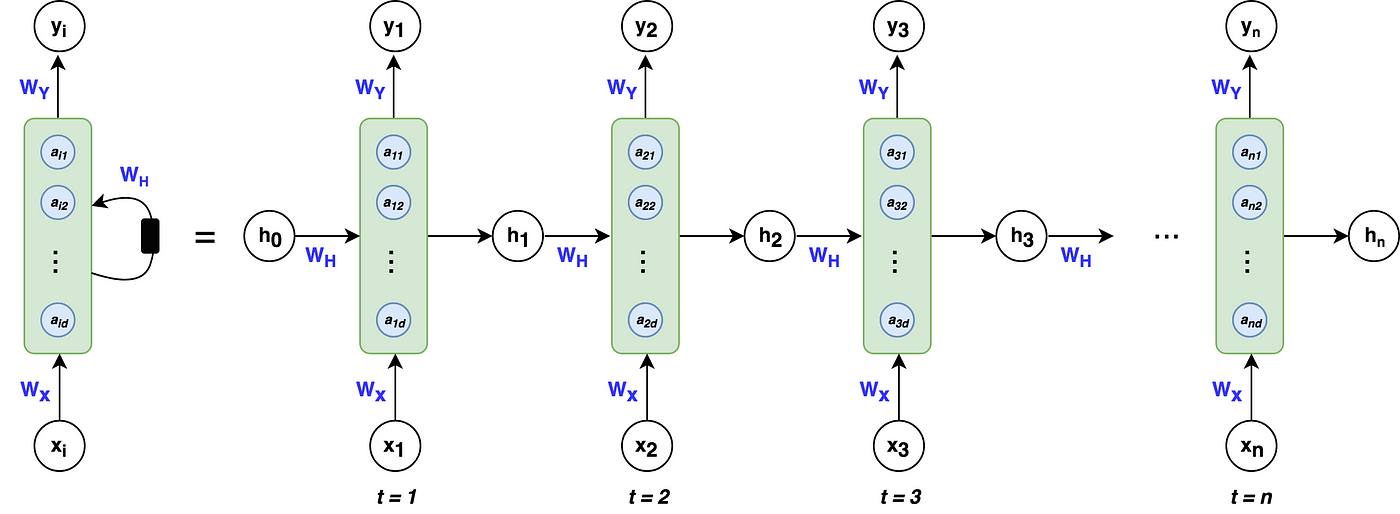
\includegraphics[width=0.8\textwidth]{resources/chapter-2-recurrentNN.png}
        \caption{Arsitektur RNN \parencite{ishwarya2024rnn}}  
        \label{fig:RNN-architecture}   
    \end{figure}


Ketika menangani data sekuensial (data teks, urutan gambar, sinyal suara, atau \textit{time series}), urutan (\textit{order}) data sangatlah penting. Contohnya, dalam pemrosesan teks, kata di posisi ke-5 memiliki konteks makna yang ditentukan oleh kata-kata sebelumnya (posisi 1--4). \textit{Vanilla RNN} adalah bentuk paling sederhana dari RNN yang menerapkan ide “menyimpan konteks” tersebut melalui sebuah \textit{hidden state} yang diperbarui di setiap langkah waktu. 

Arsitektur \textit{Vanilla RNN} dapat direpresentasikan sebagai berikut. 
\begin{enumerate} 
\item \textbf{\textit{Input} ($x_t$)}: Vektor yang merepresentasikan data pada waktu $t$. Sebagai contoh, representasi kata (\textit{word embedding}) dalam pengolahan teks, atau nilai sesuatu pada waktu $t$ dalam \textit{time series}. 
\item \textbf{\textit{Hidden state} ($H_t$)}: “Memori internal” RNN yang menampung informasi dari langkah waktu sebelumnya ($H_{t-1}$). 
\item \textbf{\textit{Output} ($y_t$)}: Vektor yang menjadi keluaran pada waktu $T$. Dalam beberapa kasus, \textit{Neural network} hanya mengeluarkan hasil di langkah terakhir. Akan tetapi pada kasus lain (misalnya \textit{language modeling}), \textit{neural network} bisa mengeluarkan hasil di setiap langkah. 
\end{enumerate}

Secara matematis, proses ini dapat direpresentasikan oleh dua persamaan utama yaitu persamaan \ref{eq:rnn-hidden-state-lengkap} dan \ref{eq:rnn-output-lengkap} dengan keterangan :
\begin{equationfloat}
\begin{equation}
\mathbf{h}_t = \phi\bigl(W_{xh}\,\mathbf{x}_t + W_{hh}\,\mathbf{h}_{t-1} + \mathbf{b}_h\bigr)
\end{equation}
\caption{\textit{Hidden state} pada \textit{Vanilla RNN}}
\label{eq:rnn-hidden-state-lengkap}
\end{equationfloat}

\begin{equationfloat}
\begin{equation}
\mathbf{y}_t = W_{hy}\,\mathbf{h}_t + \mathbf{b}_y
\end{equation}
\caption{\textit{Output} pada \textit{Vanilla RNN}}
\label{eq:rnn-output-lengkap}
\end{equationfloat}

\begin{itemize}
    \item $\mathbf{x}_t \in \mathbb{R}^d$: \textit{Input} pada waktu $t$.
    \item $\mathbf{h}_{t-1} \in \mathbb{R}^h$: \textit{Hidden state} pada waktu $t-1$.
    \item $\mathbf{W}_{xh} \in \mathbb{R}^{h \times d}$: Bobot transformasi dari \textit{input} ke \textit{hidden state}.
\item $\mathbf{W}_{hh} \in \mathbb{R}^{h \times h}$: Bobot transformasi dari \textit{hidden state} sebelumnya ke \textit{hidden state} baru.
    \item $\mathbf{b}_h \in \mathbb{R}^h$: \textit{Bias} untuk \textit{hidden state}.
    \item $\mathbf{W}_{hy} \in \mathbb{R}^{o \times h}$: Bobot transformasi dari \textit{hidden state} ke \textit{output}.
    \item $\mathbf{b}_y \in \mathbb{R}^o$: \textit{Bias} untuk \textit{output}.
    \item $\phi(\cdot)$: \textit{Activation function}.
\end{itemize}

\textit{Forward pass} dalam RNN adalah proses menghitung $h_t$ secara berurutan dari $t=1$ sampai $t=N$. Proses \textit{forward pass} dapat dimodelkan sebagai berikut: 
\begin{enumerate}
    \item Inisialisasi $\mathbf{h}_0$, umumnya sebagai vektor nol ($\mathbf{0}$).
    \item Untuk setiap waktu $t$ dalam $\{1, 2, \dots, N\}$:
 \begin{enumerate}
        \item Hitung $\mathbf{h}_t = \phi(\mathbf{W}_{xh}\mathbf{x}_t + \mathbf{W}_{hh}\mathbf{h}_{t-1} + \mathbf{b}_h)$.
        \item Hitung $\mathbf{y}_t = \mathbf{W}_{hy}\mathbf{h}_t + \mathbf{b}_y$.
  \end{enumerate}
\end{enumerate}

Setelah mendapatkan \textit{output} di setiap $T$, \textit{neural network} akan menghitung \textit{loss function} yang mengukur seberapa baik prediksi $\mathbf{y}_t$  dibandingkan dengan nilai sebenarnya $\hat{\mathbf{y}}_t$. \textit{Backward Pass} dan \textit{Backpropagation Through Time (BPTT)} Untuk melakukan \textit{training} pada RNN. Akan digunakan \textit{Backpropagation Through Time (BPTT)} yang merupakan penerapan \textit{chain rule} secara berurutan dari waktu $t=N$ “kembali” ke $t=1$. Pertama, akan dilakukan perhitungan turunan $\frac{\partial \text{Loss}}{\partial \mathbf{h}_t}$ pada setiap $t$. Selanjutnya, pada setiap langkah waktu, turunan akan dicari menggunakan \textit{chain rule} ($\frac{\partial \mathbf{h}_t}{\partial \mathbf{h}_{t-1}}$, $\frac{\partial \mathbf{h}_t}{\partial \mathbf{W}_{xh}}$, $\frac{\partial \mathbf{h}_t}{\partial \mathbf{W}_{hh}}$, dan $\frac{\partial \text{Loss}}{\partial \mathbf{y}_t}$ untuk menemukan gradien parameter ($\frac{\partial \text{Loss}}{\partial \mathbf{W}_{xh}}$, $\frac{\partial \text{Loss}}{\partial \mathbf{W}_{hh}}$, \dots)). \textit{Weight} dari setiap neuron $(\mathbf{W}_{xh}, \mathbf{W}_{hh}, \mathbf{W}_{hy}, \mathbf{b}_h, \mathbf{b}_y)$ akan diperbarui menggunakan algoritma optimisasi seperti  \textit{Stochastic Gradient Descent} (\textit{SGD}), \textit{Momentum}, atau \textit{Adam}. Seluruh iterasi ini akan diulang sampai nilai dari \textit{loss function} sudah tercapai atau sudah dapat diterima. 


Terdapat beberapa masalah yang dapat muncul pada RNN. Ketika urutan sekuens terlalu panjang, gradien yang dihitung lewat BPTT dapat mengecil ($\approx 0$) secara eksponensial sehingga \textit{weight} di langkah-langkah waktu awal hampir tidak terperbarui. Hal tersebut disebut sebagai \textit{vanishing gradient}. Terdapat pula masalah lain yang bernama \textit{exploding gradient}. Berlawanan dengan \textit{vanishing gradient}, gradien dapat tumbuh sangat besar ($\gg 1$), mengakibatkan pembaruan \textit{weight} yang ekstrem dan tidak stabil.

Vanilla RNN tidak efektif dalam hal komputasi karena prosesnya tidak dapat berjalan secara paralel. Setiap langkah waktu harus diolah satu per satu sehingga kecepatan pemrosesan menjadi relatif lambat jika dibandingkan dengan metode lain yang mendukung komputasi paralel. Kondisi ini dapat memperpanjang durasi \textit{trainig} seiring dengan meningkatnya ukuran dari \textit{dataset} serta \textit{time-length} dari data yang digunakan.



    \subsubsection{Gated RNN}
Gated RNN seperti LSTM (\textit{Long Short-Term Memory}) \parencite{Hochreiter1997} dan GRU (\textit{Gated Recurrent Unit}) \parencite{Cho2014} menggunakan gerbang (gate) untuk mengendalikan aliran informasi. LSTM sebagai contoh memiliki tiga gerbang: input gate ($i_t$), forget gate ($f_t$), dan output gate ($o_t$), serta cell state ($c_t$) yang berfungsi sebagai memori jangka panjang.

\begin{center}
\[
\mathbf{i}_t = \sigma(\mathbf{W}_{ix}\mathbf{x}_t + \mathbf{W}_{ih}\mathbf{h}_{t-1} + \mathbf{b}_i), \quad
\mathbf{f}_t = \sigma(\mathbf{W}_{fx}\mathbf{x}_t + \mathbf{W}_{fh}\mathbf{h}_{t-1} + \mathbf{b}_f)
\]
\[
\mathbf{o}_t = \sigma(\mathbf{W}_{ox}\mathbf{x}_t + \mathbf{W}_{oh}\mathbf{h}_{t-1} + \mathbf{b}_o), \quad
\mathbf{\tilde{c}}_t = \tanh(\mathbf{W}_{cx}\mathbf{x}_t + \mathbf{W}_{ch}\mathbf{h}_{t-1} + \mathbf{b}_c)
\]
\[\mathbf{c}_t = \mathbf{f}_t \odot \mathbf{c}_{t-1} + \mathbf{i}_t \odot \mathbf{\tilde{c}}_t\]
\[
\mathbf{h}_t = \mathbf{o}_t \odot \tanh(\mathbf{c}_t)
\]
\end{center}
di mana $\sigma$ adalah sigmoid dan $\odot$ adalah perkalian elemen-wise. Struktur ini membantu LSTM mempertahankan informasi penting lebih lama sehingga membuat LSTM lebih bagus untuk pemodelan \textit{time series} yang lebih kompleks. GRU menyederhanakan mekanisme ini dengan hanya menyediakan dua gerbang (update dan reset).

\subsubsection{Varian RNN lainnya }
Selain LSTM dan GRU, telah dikembangkan juga beberapa varian lainnya:
\begin{enumerate}
\item \textbf{Bi-directional RNN} \\
Melakukan \textit{processing input} dari dua arah (depan-belakang).
\item \textbf{Stacked RNN} \\
Menggunakan beberapa lapisan RNN sehingga model dapat mempelajari representasi yang lebih kompleks
\end{enumerate}
  \subsection{Transformer}
Transformer adalah arsitektur yang menghilangkan ketergantungan pada koneksi berulang (\textit{recurrent connections}) seperti pada RNN. Dengan menggunakan mekanisme perhatian (\textit{attention}) sebagai komponen utama, Transformer dapat memodelkan hubungan antar elemen sekuens tanpa harus memprosesnya secara serial, sehingga pelatihan dapat diparalelisasi \parencite{Vaswani2017}.

Inti dari Transformer adalah mekanisme \textit{attention} yang memungkinkan model untuk “memperhatikan” bagian \textit{input} yang paling relevan ketika memproses sebuah token tertentu. Hal ini memudahkan penangkapan hubungan jangka panjang dalam data sekuensial tanpa mengalami masalah \textit{vanishing gradient}.

\subsubsection{Positional Encoding}
Untuk memberikan informasi posisi token dalam sekuens, Transformer menggunakan \textit{positional encoding}, yang menambahkan embedding posisi ke embedding token. Pendekatan ini memungkinkan model untuk membedakan posisi relatif antar token, sehingga hubungan temporal atau urutan data dapat ditangkap.

\begin{center}
\[
\text{PE}_{(pos,2i)} = \sin\left(\frac{pos}{10000^{2i/d_{model}}}\right), \quad
\text{PE}_{(pos,2i+1)} = \cos\left(\frac{pos}{10000^{2i/d_{model}}}\right)
\]
\end{center}

di mana $pos$ adalah indeks posisi token dalam sekuens dan $i$ mengindeks dimensi embedding. Rumus ini menghasilkan pola sinusoidal yang unik untuk setiap posisi, memungkinkan model mempelajari makna posisi relatif secara implisit.

    \subsubsection{Attention Mechanism}
Mekanisme perhatian \parencite{Bahdanau2015,Luong2015} dapat dipandang sebagai fungsi yang memetakan query (Q) dan pasangan key-value (K, V) menjadi suatu keluaran. Bentuk paling umum adalah \textit{Scaled Dot-Product Attention}:

\begin{center}
\[
\text{Attention}(Q,K,V) = \text{softmax}\left(\frac{QK^\top}{\sqrt{d_k}}\right)V
\]
\end{center}
di mana \( d_k \) adalah dimensi key. Fungsi ini memberikan bobot lebih besar pada elemen input yang relevan sesuai dengan query yang diberikan. Dengan multi-head attention, beberapa set (Q, K, V) digunakan secara paralel, sehingga model dapat belajar jenis relasi yang berbeda pada waktu yang sama.

    \subsubsection{Core Transformer Architecture}
Arsitektur inti Transformer terdiri atas \textit{encoder} dan \textit{decoder}. \textit{Encoder } mengubah input menjadi representasi fitur-fitur, sedangkan decoder menggunakan representasi tersebut untuk menghasilkan output secara autoregresif.Setiap lapisan \textit{encoder} memiliki dua sub-lapisan: \textit{Multi-Head Self-Attention} dan \textit{Feed-Forward Network} (FFN). 
\begin{enumerate}
\item Multi-head self-attention \\
Mengaplikasikan \textit{attention} pada input itu sendiri (self-attention) untuk menangkap hubungan antar token dalam sekuens.
\item Position-wise feed-forward network \\
Sebuah Multi-layer perceptron yang diterapkan secara independen pada setiap posisi token.
\end{enumerate}

Setelah sub-lapisan ini, dilakukan \textit{residual connection} dan \textit{layer normalization} \parencite{Vaswani2017}. Secara matematis, jika \textbf{H} adalah masukan dari lapisan, maka satu lapisan Transformer akan  melakukan:
\begin{center}
\[
\mathbf{H}' = \text{LayerNorm}\left(\mathbf{H} + \text{MultiHeadAttention}(\mathbf{H},\mathbf{H},\mathbf{H})\right)
\]
\[
\mathbf{H}^{\star} = \text{LayerNorm}\left(\mathbf{H}' + \text{FFN}(\mathbf{H}')\right)
\]
\end{center}

Decoder memiliki struktur serupa tetapi juga lebih berfokus kepada \textit{output encoder} serta \textit{masking} pada \textit{self-attention}untuk mencegah model “melihat” token masa depan saat memprediksi token saat ini.

Salah satu tantangan pada Transformer adalah kompleksitas komputasi yang mencapai $O(T^2)$ untuk panjang sekuens $T$. Pada sekuens yang sangat panjang, ini dapat menjadi masalah. Sebagai perbandingan, RNN seperti LSTM atau GRU memproses data secara serial, namun lebih sulit diparalelisasi dan kurang efektif dalam menangkap dependensi jangka panjang. Transformer mengatasi masalah ini melalui mekanisme \textit{attention} yang dapat menjangkau seluruh sekuens secara langsung, meskipun dengan beban komputasi kuadratik.
  \subsubsection{Extended Transformer}  
Berbagai varian dari Transformer telah dikembangkan untuk mengatasi isu efisiensi, diperlukannya konteks yang lebih panjang, dan domain khusus:
\begin{enumerate}
\item \textbf{Longformer, Reformer:} Menggunakan \textit{attention} yang lebih efisien (\textit{sparse } atau berbasis hashing) untuk mengurangi kompleksitas.
\item \textbf{Vision Transformer (ViT):} Mengaplikasikan \textit{attention} pada patch citra.
\item \textbf{BERT, GPT:} Spesialisasi dalam pemahaman bahasa (BERT) dan generasi teks (GPT).
\end{enumerate}
 \subsubsection{Temporal Fusion Transformer}
Temporal Fusion Transformer \parencite{Lim2020} adalah varian Transformer yang dirancang khusus untuk peramalan deret waktu \textit{multi-horizon}. TFT menggabungkan ide \textit{attention} dengan mekanisme \textit{gating} dan \textit{Gated Residual Network} untuk memilih variabel yang relevan dan mempelajari hubungan variabel antar waktu.

Pada TFT, Variable Selection Network (VSN) digunakan untuk mengekstrak fitur yang paling penting, sementara Gated Residual Network (GRN) membantu mengontrol aliran informasi dan mengatasi overfitting.
    
\begin{center}
\[
\mathbf{h}^{\text{selected}} = \text{VSN}(\mathbf{X})
\]
\[
\mathbf{h}^{\text{processed}} = \text{GRN}(\mathbf{h}^{\text{selected}})
\]
\[
\mathbf{H}_{att} = \text{MultiHeadAttention}(Q=\mathbf{h}^{\text{processed}},K=\mathbf{h}^{\text{processed}},V=\mathbf{h}^{\text{processed}})
\]
\[
\mathbf{Z}_{final} = \text{GRN}(\mathbf{H}_{att})
\]

\end{center}
    
\section{Evaluation Metrics}
\section{Penelitian Terkait}
\blindtext
